\chapter{Updating the ND280 fit for 2018+}
The official 2017 analysis presented in \autoref{chap:ND280} used data from T2K runs 2 through 6, which was collected between 2010 and 2015. It was largely developed for the 2015 analyses, with an inconsistent 0$\pi$, 1$\pi$ and Other selection for \numu in FHC, and 1Track and NTrack for \numubar and \numu in RHC. Primarily due to low statistics and the 1Trk/NTrk selection, the posterior predictive p-values for the anti-neutrino samples were generally uninformative---centered around 0.5---implying not much could be said about the health of T2K anti-neutrino modelling.

For the upcoming 2018+ analyses, the near-detector fit has several updates which further pushes the uncertainties down for T2K-SK analysers, which will be presented in this chapter.

\section{Adding run 7 and 8 data}
Adding to the run 2 to 6 data, T2K has been collecting POT steadily since 2015, making it possible to refine the selections and update the binning for increased sensitivity. As previously shown in \autoref{fig:t2k_pot}, almost double the amount of protons-on-target were accumulated in run 7 (RHC) and 8 (FHC) due to an increasing beam power, culminating at nearly 500 kW.

\autoref{tab:pot_2018} shows the run-by-run breakdown of the data and generated Monte-Carlo POT, directly comparable to the 2017 equivalent for run 2 to 6 in \autoref{tab:pot_2017}. The amount of FHC data increased by 99\% and RHC data by 63\%.
\begin{table}[h]
	\centering
	\begin{tabular}{ l c c c }
		\hline
		\hline
		Run &  \multicolumn{3}{c}{POT (E+19)} \\
		    & 	Data & MC & Sand \\
		\hline
		2a  & 3.59337    & 92.3937     & 3.7132  \\
		2w  & 4.33765    & 120.341     & 4.00035 \\
		\hline
		3b  & 2.1705     & 44.7864     & 2.35053 \\
		3c  & 13.6398    & 263.227     & 13.1337 \\
		\hline
		4a  & 17.8271    & 349.96      & 17.4125 \\
		4w  & 16.4277    & 226.216     & 15.9801 \\
		\hline
		5   & 4.3468     & 229.627     & 9.07403 \\
		\hline
		6b  & 12.7301    & 141.74      & 25.9187 \\
		6c  & 5.07819    & 52.7562     & 10.4626 \\
		6d  & 7.75302    & 68.83       & 15.8059 \\
		6e  & 8.51429    & 85.9439     & 17.2691 \\
		\hline
		7   & 24.3683	 & 337.059     & 50.3961 \\
		\hline
		8a  & 41.4909	 & 363.054	   & 40.1875 \\
		8w  & 15.8053    & 264.115 	   & 16.1263 \\
		\hline
		Total FHC & 115.29232 & 1724.0931 &  112.09418 \\
		Total RHC & 62.791 	  & 915.9561  &  127.92643 \\
		\hline
		\hline
		Total 	  & 178.08332 & 2640.0492 &  240.83061 \\
		\hline
		\hline
		Total FHC x2017 & 1.9876 & --- & --- \\
		Total RHC x2017 & 1.6276 & --- & --- \\
		Total x2017 	& 1.8438 & --- & --- \\
		\hline
		\hline
	\end{tabular}
	\caption{Counted and generated proton-on-targets for the T2K ND280 2018+ analysis}
	\label{tab:pot_2018}
\end{table}

\section{Selections}
For the selection update we only change the RHC sample from 1Track/NTrack to 0$\pi$, 1$\pi$ and Other. The FHC selection remains identical to as was presented in \autoref{sec:numu_sel}. The pion counting for the RHC sample matches that of \autoref{sec:numu_sel}, using either the TPC, FGD Michel electron or FGD isolated track reconstruction for the pion tag. 

In summary, the TPC pion PID requires that the track (with $p_{reco}<500\text{ MeV}$) has a MIP likelihood of $\mathcal{L}_{MIP} > 0.8$ (\autoref{eq:tpc_track_mip}) and a pion likelihood of $\mathcal{L}_\pi > 0.3$. The FGD is also used to search for pion-like deposits using a Michel electron tag which searches for a time-delayed FGD hit cluster, and a FGD reconstructed pion tag using an optimised pion pull cut for forwards-going events ($|\cos\theta_{\pi,\nu}|>0.3$).

The only difference in the likelihood cuts from \autoref{sec:ND280:sel} is for the $\mu^+$ selection, which in \autoref{sec:numubar_sel} required $0.1 < \mathcal{L}_\mu < 0.7$. The upper bound at 0.7 was present to reject low energy $\mu^-$ from \numu RHC interactions, which was discarded for this analysis after it gave a 4\% increase in efficiency with negligible purity change. The $\mu^-$ criteria for the \numu in RHC selection did not change and still requires a MIP-like track with $0.1 < \mathcal{L}_\mu < 0.8$.

Since the FHC selection is unchanged, the efficiency and purities are very similar and here we only compare FGD1 CC0$\pi$ in 2018 to 2017 in \autoref{fig:fgd1_cc0pi_eff_2017_2018}, and refer to \autoref{tab:eff_pur_summary_2018} for the summary.
\begin{figure}[h]
	\centering
	\caption*{2018 analysis}
	\begin{subfigure}[t]{\textwidth}
		\centering
	\begin{subfigure}[t]{0.4\textwidth}
		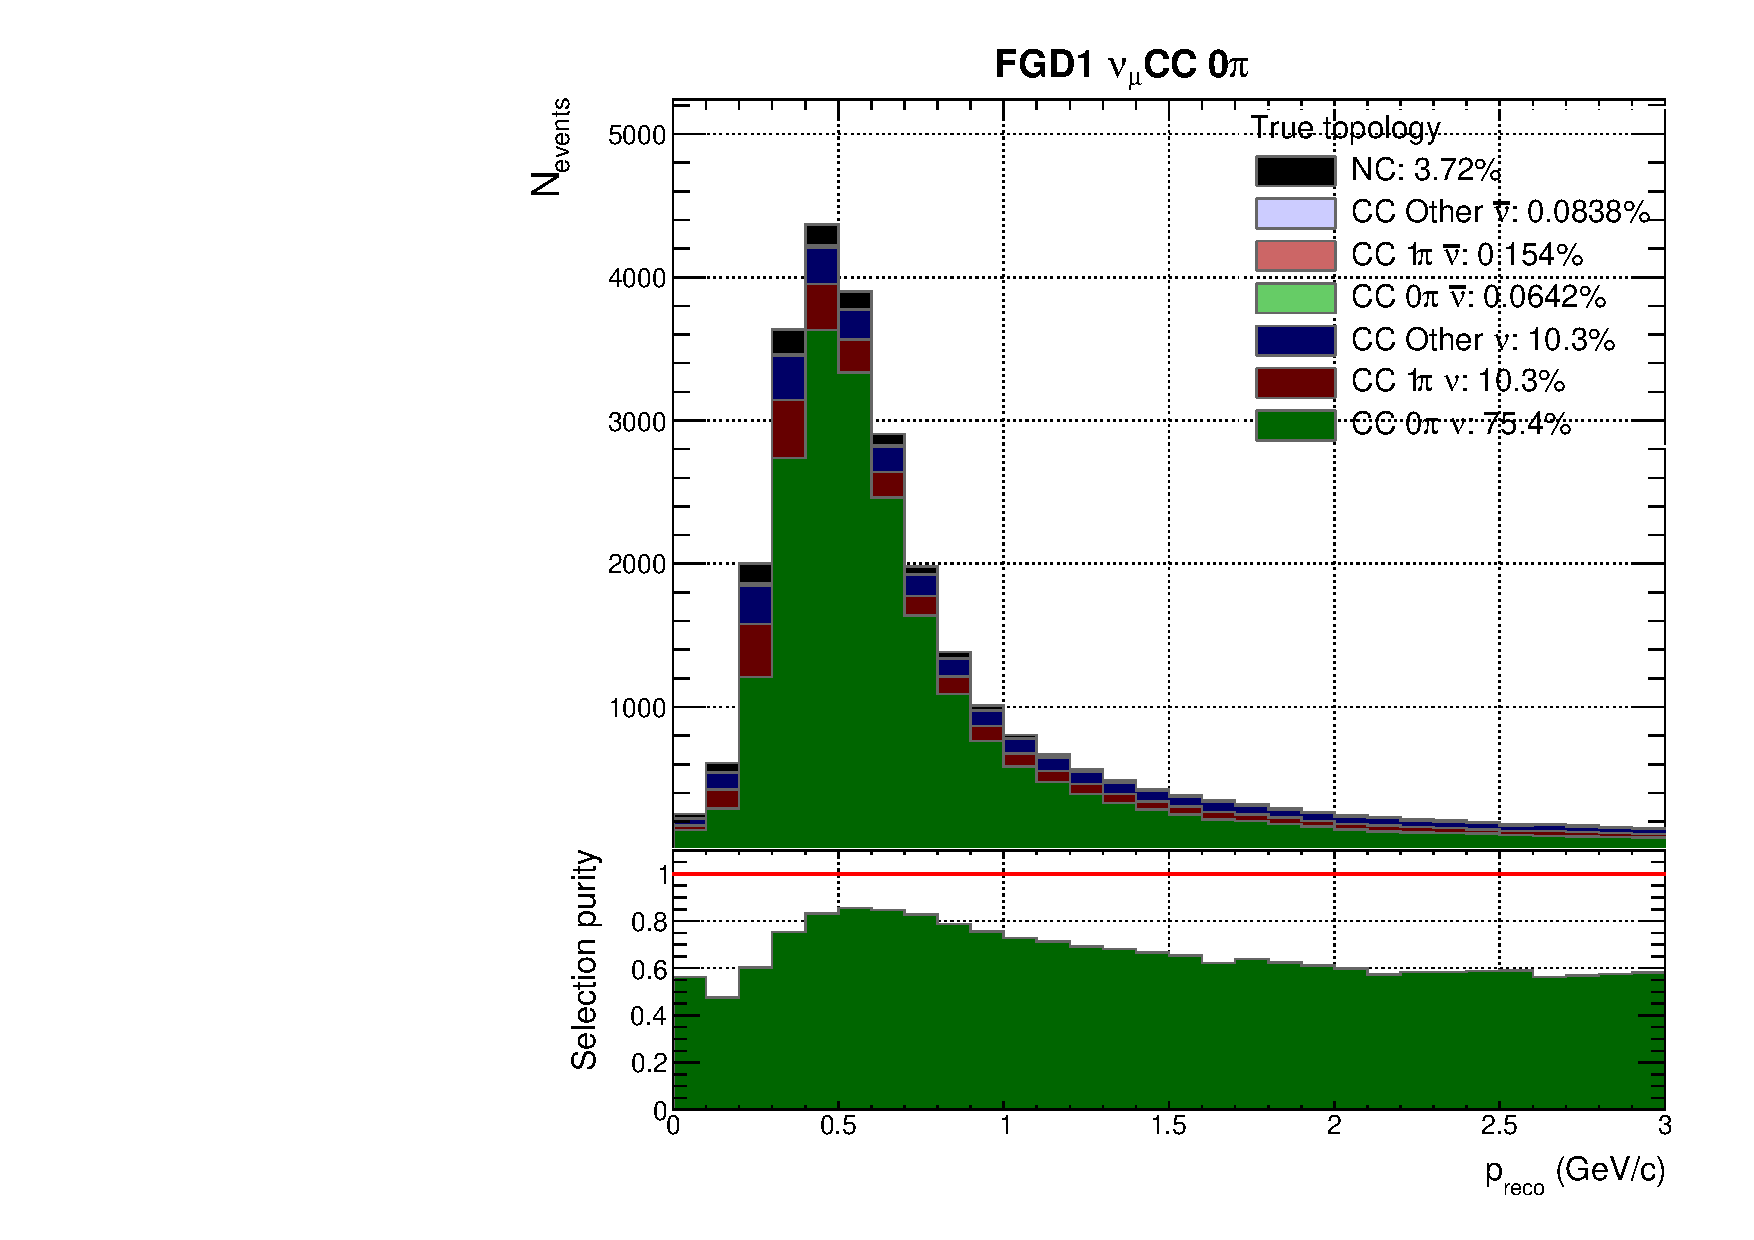
\includegraphics[width=\textwidth,page=1, trim={0mm 0mm 0mm 9mm}, clip]{figures/mach3/2018/Selection/2018_FullNoRedNDmatrix_rebin_verbose_may_diagnostics}
		\caption{Efficiency}
	\end{subfigure}
	\begin{subfigure}[t]{0.4\textwidth}
		\includegraphics[width=\textwidth,page=2, trim={0mm 0mm 0mm 9mm}, clip]{figures/mach3/2018/Selection/2018_FullNoRedNDmatrix_rebin_verbose_may_diagnostics}
		\caption{Purity}
	\end{subfigure}
\end{subfigure}

	\begin{subfigure}[t]{\textwidth}
		\centering
		\caption*{2017 analysis}
	\begin{subfigure}[t]{0.4\textwidth}
	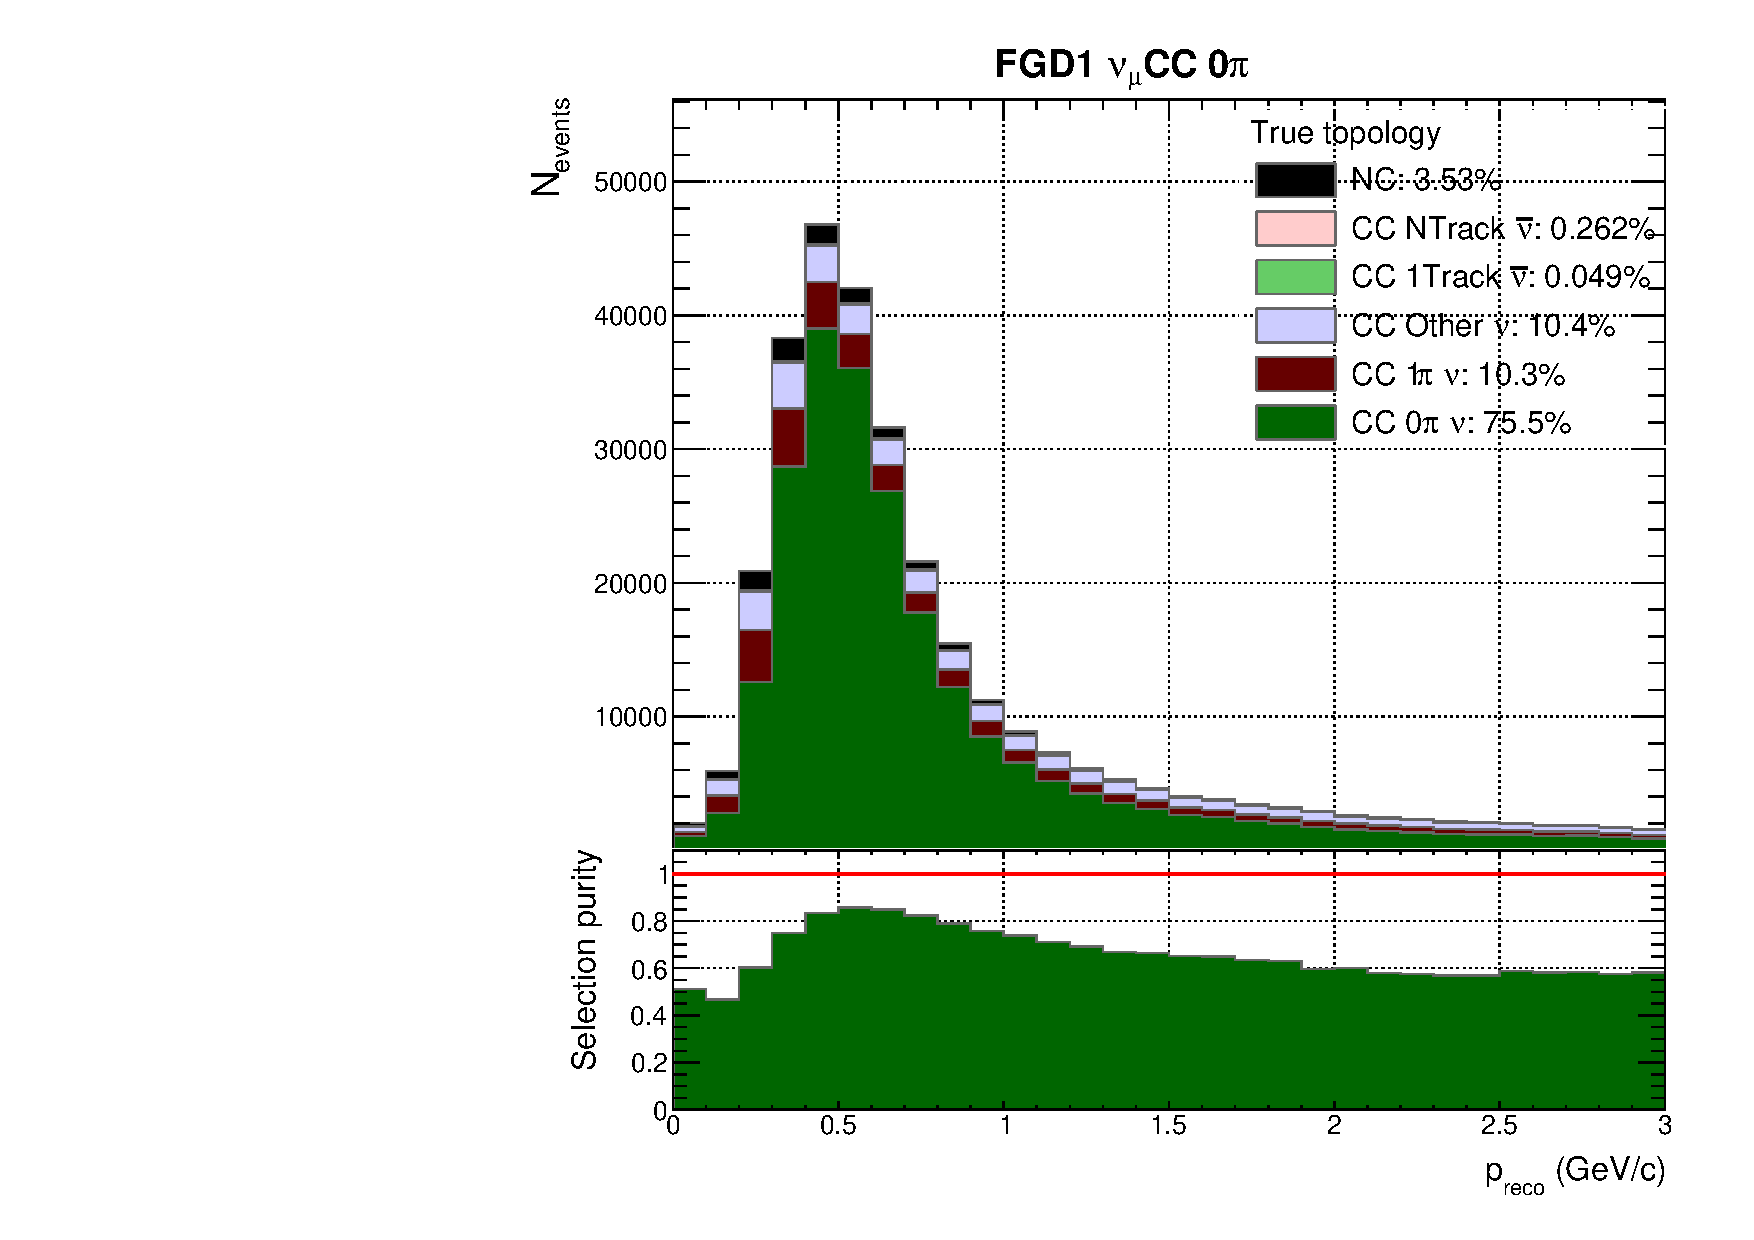
\includegraphics[width=\textwidth,page=1, trim={0mm 0mm 0mm 9mm}, clip]{figures/mach3/selection/2017b_Diag_WithSelection}
	\caption{Efficiency}
\end{subfigure}
\begin{subfigure}[t]{0.4\textwidth}
	\includegraphics[width=\textwidth,page=2, trim={0mm 0mm 0mm 9mm}, clip]{figures/mach3/selection/2017b_Diag_WithSelection}
	\caption{Purity}
\end{subfigure}
\end{subfigure}
\caption{FGD1 0$\pi$ efficiencies and purities for 2017 and 2018 analyses}
\label{fig:fgd1_cc0pi_eff_2017_2018}
\end{figure}

For the new \numu and \numubar RHC samples we study the efficiencies and purities in the same way as \autoref{sec:ND280:sel}, using unweighted raw Monte-Carlo events.

\subsection{\numubar in RHC}
The CC0$\pi$ RHC selections are much the same as the 2017 1Track selection, and as such the purity in \autoref{fig:numubar_cc0pi_topology} is almost identical to \autoref{fig:ccnubar1trk_topology}. Both FGDs have similar purities and the largest contamination is right-sign single pion events in which the pion is missed, at about 9.5\%. The NC contribution is 5.1\% and the total wrong-sign contribution is $\sim5\%$, similar to the 1Trk selection. The difference comes primarily from the removed upper bound on the muon likelihood cut. Moving up in momentum, the purity reduces to about 60\% from 85\% at the event peak.
\begin{figure}[h]
	\begin{subfigure}[t]{0.49\textwidth}
		\includegraphics[width=\textwidth,page=13, trim={0mm 0mm 0mm 9mm}, clip]{figures/mach3/2018/Selection/2018_FullNoRedNDmatrix_rebin_verbose_may_diagnostics}
		\caption{FGD1}
	\end{subfigure}
	\begin{subfigure}[t]{0.49\textwidth}
		\includegraphics[width=\textwidth,page=19, trim={0mm 0mm 0mm 9mm}, clip]{figures/mach3/2018/Selection/2018_FullNoRedNDmatrix_rebin_verbose_may_diagnostics}
		\caption{FGD2}
	\end{subfigure}
	\caption{Breakdown of \numubar CC0$\pi$ selection events' true event topology for FGD1 and FGD2 }
	\label{fig:numubar_cc0pi_topology}
\end{figure}

\autoref{fig:numubar_cc0pi_muon} shows the muon tagging efficiency, which again is comparable to the 1Trk equivalent in \autoref{fig:ccnubar1trk_muon}. The largest mis-id comes from $\pi^+$ being reconstructed as the muon, and the wrong-sign contamination is small. At $\sim1.5\text{ GeV}$ we see the characteristic proton bump, in which the dE/dx of a proton is very similar to that of a muon, causing it to be the selected highest momentum positive track with a muon likelihood.
\begin{figure}[h]
	\begin{subfigure}[t]{0.49\textwidth}
		\includegraphics[width=\textwidth,page=14, trim={0mm 0mm 0mm 9mm}, clip]{figures/mach3/2018/Selection/2018_FullNoRedNDmatrix_rebin_verbose_may_diagnostics}
		\caption{FGD1}
	\end{subfigure}
	\begin{subfigure}[t]{0.49\textwidth}
		\includegraphics[width=\textwidth,page=20, trim={0mm 0mm 0mm 9mm}, clip]{figures/mach3/2018/Selection/2018_FullNoRedNDmatrix_rebin_verbose_may_diagnostics}
		\caption{FGD2}
	\end{subfigure}
	\caption{Breakdown of \numubar CC0$\pi$ selection events' true lepton candidate for FGD1 and FGD2}
	\label{fig:numubar_cc0pi_muon}
\end{figure}

Moving to the 1$\pi$ \numubar selection, the purity is shown in \autoref{fig:numubar_cc1pi_topology}. The \numubar RHC selection is not much worse than for the \numu FHC equivalent in \autoref{fig:cc1pi_topology}, reaching an overall purity of $\sim 51\%$, with FGD2 slightly worse. The wrong-sign contamination is significant at 25\%, coming from a $\pi^+$ in a CC1$\pi^+$ or CC DIS event being reconstructed as the muon candidate, and the $\mu^-$ reconstructed as the $\pi^-$. The right-sign CCOther contamination is about 10\%, owing mostly to one or several missed $\pi$. We again see the CC0$\pi$ \numu peak at 1.5 GeV, where the proton (likely from a CCQE or 2p2h interaction) is reconstructed as the $\mu^+$.
\begin{figure}[h]
	\begin{subfigure}[t]{0.49\textwidth}
		\includegraphics[width=\textwidth,page=15, trim={0mm 0mm 0mm 9mm}, clip]{figures/mach3/2018/Selection/2018_FullNoRedNDmatrix_rebin_verbose_may_diagnostics}
		\caption{FGD1}
	\end{subfigure}
	\begin{subfigure}[t]{0.49\textwidth}
		\includegraphics[width=\textwidth,page=21, trim={0mm 0mm 0mm 9mm}, clip]{figures/mach3/2018/Selection/2018_FullNoRedNDmatrix_rebin_verbose_may_diagnostics}
		\caption{FGD2}
	\end{subfigure}
	\caption{Breakdown of \numubar CC1$\pi$ selection events' true event topology for FGD1 and FGD2 }
	\label{fig:numubar_cc1pi_topology}
\end{figure}

\autoref{fig:numubar_cc1pi_muon} shows the muon tagging efficiency, which in the event peak sits at 80\% and decreases to 50\% with increasing $p_{\text{reco}}$. Tagging the right-sign pion as the lepton candidate happens 20\% of the time, and protons about 15\% of the time, making up a large fraction of mis-identification. However, the 1$\pi$ selection is still almost 10\% more efficient and pure than the old CCNTrack selection.
\begin{figure}[h]
	\begin{subfigure}[t]{0.49\textwidth}
		\includegraphics[width=\textwidth,page=16, trim={0mm 0mm 0mm 9mm}, clip]{figures/mach3/2018/Selection/2018_FullNoRedNDmatrix_rebin_verbose_may_diagnostics}
		\caption{FGD1}
	\end{subfigure}
	\begin{subfigure}[t]{0.49\textwidth}
		\includegraphics[width=\textwidth,page=22, trim={0mm 0mm 0mm 9mm}, clip]{figures/mach3/2018/Selection/2018_FullNoRedNDmatrix_rebin_verbose_may_diagnostics}
		\caption{FGD2}
	\end{subfigure}
	\caption{Breakdown of \numubar CC1$\pi$ selection events' true lepton candidate for FGD1 and FGD2}
	\label{fig:numubar_cc1pi_muon}
\end{figure}

Finally \autoref{fig:numubar_ccOth_topology} shows the purity of the \numubar CCOther selection, which collects all \numubar CC events that weren't classified as CC0$\pi$ or CC1$\pi$. As with the \numu equivalent selection, the sample suffers from low purity due to broken tracks and secondary interactions, leading to a misreconstructed number of pions in the event. It also has a high NC contamination due to collecting high pion multiplicity events, causing a pion to be reconstructed as a muon in the TPC. The selection has an almost equal efficiency for \numubar CCOther events as it does for \numu CCOther events, and in FGD2 it's indeed more pure of wrong-sign events. At low momentum, the purity is close to zero, being swamped by wrong-sign 0$\pi$ events in which the low momentum $\mu^-$ is identified as a $\mu^+$, owing to the changed likelihood cut which used to remove such events. The wrong-sign 0$\pi$ and 1$\pi$ purity largely vanishes above 500 MeV and the wrong sign component is almost exclusively \numu CCOther.
\begin{figure}[h]
	\begin{subfigure}[t]{0.49\textwidth}
		\includegraphics[width=\textwidth,page=17, trim={0mm 0mm 0mm 9mm}, clip]{figures/mach3/2018/Selection/2018_FullNoRedNDmatrix_rebin_verbose_may_diagnostics}
		\caption{FGD1}
	\end{subfigure}
	\begin{subfigure}[t]{0.49\textwidth}
		\includegraphics[width=\textwidth,page=23, trim={0mm 0mm 0mm 9mm}, clip]{figures/mach3/2018/Selection/2018_FullNoRedNDmatrix_rebin_verbose_may_diagnostics}
		\caption{FGD2}
	\end{subfigure}
	\caption{Breakdown of \numubar CCOther selection events' true event topology for FGD1 and FGD2 }
	\label{fig:numubar_ccOth_topology}
\end{figure}

The muon tagging efficiency is shown in \autoref{fig:numubar_ccOth_muon}, which echoes the conclusions above. The efficiency is below 50\% and has almost equal parts proton tagging and $\pi^+$ tagging as contaminants. The wrong sign tagging happens primarily at low momentum, in which the charge is wrongly reconstructed in the magnetic field.
\begin{figure}[h]
	\begin{subfigure}[t]{0.49\textwidth}
		\includegraphics[width=\textwidth,page=18, trim={0mm 0mm 0mm 9mm}, clip]{figures/mach3/2018/Selection/2018_FullNoRedNDmatrix_rebin_verbose_may_diagnostics}
		\caption{FGD1}
	\end{subfigure}
	\begin{subfigure}[t]{0.49\textwidth}
		\includegraphics[width=\textwidth,page=24, trim={0mm 0mm 0mm 9mm}, clip]{figures/mach3/2018/Selection/2018_FullNoRedNDmatrix_rebin_verbose_may_diagnostics}
		\caption{FGD2}
	\end{subfigure}
	\caption{Breakdown of \numubar CCOther selection events' true lepton candidate for FGD1 and FGD2}
	\label{fig:numubar_ccOth_muon}
\end{figure}

\subsection{\numu in RHC}
As with the \numubar CC0$\pi$ selection, the \numu RHC CC0$\pi$ selection is largely identical to the 1Track equivalent in the 2017 analysis. The purity in \autoref{fig:numurhc_cc0pi_topology} is slightly above 53\%, with large contamination from right-sign 1$\pi$ and Other interactions, with the wrong-sign background making up 8\%, slightly less than the 1Track case. The NC contamination is almost identical at 9\%. We note the purity above 600 MeV stabilises at about 60\%.
\begin{figure}[h]
	\begin{subfigure}[t]{0.49\textwidth}
		\includegraphics[width=\textwidth,page=25, trim={0mm 0mm 0mm 9mm}, clip]{figures/mach3/2018/Selection/2018_FullNoRedNDmatrix_rebin_verbose_may_diagnostics}
		\caption{FGD1}
	\end{subfigure}
	\begin{subfigure}[t]{0.49\textwidth}
		\includegraphics[width=\textwidth,page=31, trim={0mm 0mm 0mm 9mm}, clip]{figures/mach3/2018/Selection/2018_FullNoRedNDmatrix_rebin_verbose_may_diagnostics}
		\caption{FGD2}
	\end{subfigure}
	\caption{Breakdown of \numu RHC CC0$\pi$ selection events' true event topology for FGD1 and FGD2 }
	\label{fig:numurhc_cc0pi_topology}
\end{figure}

The muon tagging efficiency is shown in \autoref{fig:numurhc_cc0pi_muon}, where we note 90\% efficiency above 1 GeV. At the event peak the efficiency sits at 65\%, leading to overall 77\%. In and below the event peak the main contamination is from $\pi^-$ (12\%) and as we go down in momentum the wrong-sign contributions increase due to bad sign reconstruction in the magnet. At low momentum the wrong-sign component is $\times10$ larger than the right-sign.
\begin{figure}[h]
	\begin{subfigure}[t]{0.49\textwidth}
		\includegraphics[width=\textwidth,page=26, trim={0mm 0mm 0mm 9mm}, clip]{figures/mach3/2018/Selection/2018_FullNoRedNDmatrix_rebin_verbose_may_diagnostics}
		\caption{FGD1}
	\end{subfigure}
	\begin{subfigure}[t]{0.49\textwidth}
		\includegraphics[width=\textwidth,page=32, trim={0mm 0mm 0mm 9mm}, clip]{figures/mach3/2018/Selection/2018_FullNoRedNDmatrix_rebin_verbose_may_diagnostics}
		\caption{FGD2}
	\end{subfigure}
	\caption{Breakdown of \numu RHC CC0$\pi$ selection events' true lepton candidate for FGD1 and FGD2}
	\label{fig:numurhc_cc0pi_muon}
\end{figure}

The CC1$\pi$ purity is shown in \autoref{fig:numurhc_cc1pi_topology}, in which we again see a large wrong-sign contribution at low momentum. The purity is roughly 43\% overall, and a meagre 20\% in the event peak. The right-sign CCOther amount is constant with momentum, making up almost 1/3 at the higher end.
\begin{figure}[h]
	\begin{subfigure}[t]{0.49\textwidth}
		\includegraphics[width=\textwidth,page=27, trim={0mm 0mm 0mm 9mm}, clip]{figures/mach3/2018/Selection/2018_FullNoRedNDmatrix_rebin_verbose_may_diagnostics}
		\caption{FGD1}
	\end{subfigure}
	\begin{subfigure}[t]{0.49\textwidth}
		\includegraphics[width=\textwidth,page=33, trim={0mm 0mm 0mm 9mm}, clip]{figures/mach3/2018/Selection/2018_FullNoRedNDmatrix_rebin_verbose_may_diagnostics}
		\caption{FGD2}
	\end{subfigure}
	\caption{Breakdown of \numu RHC CC1$\pi$ selection events' true event topology for FGD1 and FGD2 }
	\label{fig:numurhc_cc1pi_topology}
\end{figure}

The muon tagging efficiency in \autoref{fig:numurhc_cc1pi_muon} performs similarly to the NTrack selection at 65\%. At the event peak the efficiency is barely 20\% but increases steadily to 85\% at higher momentum where to wrong-sign component vanishes. The total wrong-sign contribution is 12\% but is dominant at low momentum. The $\pi^-$ contribution is sizeable at 22\%, which also dies off at higher momentum.
\begin{figure}[h]
	\begin{subfigure}[t]{0.49\textwidth}
		\includegraphics[width=\textwidth,page=28, trim={0mm 0mm 0mm 9mm}, clip]{figures/mach3/2018/Selection/2018_FullNoRedNDmatrix_rebin_verbose_may_diagnostics}
		\caption{FGD1}
	\end{subfigure}
	\begin{subfigure}[t]{0.49\textwidth}
		\includegraphics[width=\textwidth,page=34, trim={0mm 0mm 0mm 9mm}, clip]{figures/mach3/2018/Selection/2018_FullNoRedNDmatrix_rebin_verbose_may_diagnostics}
		\caption{FGD2}
	\end{subfigure}
	\caption{Breakdown of \numu RHC CC1$\pi$ selection events' true lepton candidate for FGD1 and FGD2}
	\label{fig:numurhc_cc1pi_muon}
\end{figure}

The \numu RHC CCOther selection has relatively good purity in \autoref{fig:numurhc_ccOth_topology}, overall 60.4\%. At low momentum the NC contribution is the largest, which is also the largest background overall at 13\%. Interestingly, the 0$\pi$ selection contaminates the sample 10\% and is the second largest contamination.
\begin{figure}[h]
	\begin{subfigure}[t]{0.49\textwidth}
		\includegraphics[width=\textwidth,page=29, trim={0mm 0mm 0mm 9mm}, clip]{figures/mach3/2018/Selection/2018_FullNoRedNDmatrix_rebin_verbose_may_diagnostics}
		\caption{FGD1}
	\end{subfigure}
	\begin{subfigure}[t]{0.49\textwidth}
		\includegraphics[width=\textwidth,page=35, trim={0mm 0mm 0mm 9mm}, clip]{figures/mach3/2018/Selection/2018_FullNoRedNDmatrix_rebin_verbose_may_diagnostics}
		\caption{FGD2}
	\end{subfigure}
	\caption{Breakdown of \numu RHC CCOther selection events' true event topology for FGD1 and FGD2 }
	\label{fig:numurhc_ccOth_topology}
\end{figure}

The corresponding muon efficiency is shown in \autoref{fig:numurhc_ccOth_muon}, where we see close to zero at low momentum. In this region the electron is the principal background but dies down above 200 MeV. After that the $\pi^-$ is the only competing background at $\sim20\%$. The overall efficiency is 68\% and stabilises at 1 GeV.
\begin{figure}[h]
	\begin{subfigure}[t]{0.49\textwidth}
		\includegraphics[width=\textwidth,page=30, trim={0mm 0mm 0mm 9mm}, clip]{figures/mach3/2018/Selection/2018_FullNoRedNDmatrix_rebin_verbose_may_diagnostics}
		\caption{FGD1}
	\end{subfigure}
	\begin{subfigure}[t]{0.49\textwidth}
		\includegraphics[width=\textwidth,page=36, trim={0mm 0mm 0mm 9mm}, clip]{figures/mach3/2018/Selection/2018_FullNoRedNDmatrix_rebin_verbose_may_diagnostics}
		\caption{FGD2}
	\end{subfigure}
	\caption{Breakdown of \numu RHC CCOther selection events' true lepton candidate for FGD1 and FGD2}
	\label{fig:numurhc_ccOth_muon}
\end{figure}

A summary of all selections' efficiency and purities is shown in \autoref{tab:eff_pur_summary_2018}.
\begin{table}[h]
	\centering
	\begin{tabular}{ l | c c }
		\hline
		\hline
		Selection 					   & Efficiency (\%) & Purity (\%) \\ 
		\hline
		\FGDCCNoPi{1}{\numu}           & 93.5  & 75.4  \\% \hline
		\FGDCCNoPi{2}{\numu}           & 92.8  & 73.2  \\% \hline
		\hline
		\FGDCCOnePi{1}{\numu}          & 83.4  & 56.6  \\% \hline
		\FGDCCOnePi{2}{\numu}          & 82.8  & 56.4  \\% \hline
		\hline
		\FGDCCOther{1}{\numu}          & 73.0  & 64.6  \\% \hline
		\FGDCCOther{2}{\numu}          & 73.3  & 64.6  \\% \hline
		\hline
		\FGDCCNoPi{1}{\numubar}           & 89.0  & 74.9  \\% \hline
		\FGDCCNoPi{2}{\numubar}           & 87.7  & 73.9  \\% \hline
		\hline
		\FGDCCOnePi{1}{\numubar}          & 65.1  & 53.7  \\% \hline
		\FGDCCOnePi{2}{\numubar}          & 61.2  & 49.8  \\% \hline
		\hline
		\FGDCCOther{1}{\numubar}          & 44.0  & 24.0  \\% \hline
		\FGDCCOther{2}{\numubar}          & 41.8  & 23.2  \\% \hline
		\hline		
		\FGDCCNoPi{1}{\numu RHC}           & 79.0  & 55.3  \\% \hline
		\FGDCCNoPi{2}{\numu RHC}           & 77.4  & 52.9 \\% \hline
		\hline
		\FGDCCOnePi{1}{\numu RHC}          & 65.3  & 42.8  \\% \hline
		\FGDCCOnePi{2}{\numu RHC}          & 66.6  & 43.0  \\% \hline
		\hline
		\FGDCCOther{1}{\numu RHC}          & 68.5  & 60.4  \\% \hline
		\FGDCCOther{2}{\numu RHC}          & 68.7  & 60.7  \\% \hline
		\hline
		\hline
	\end{tabular}
	\caption{Efficiency and purity summary for all selections with the range $0 < p_{reco} < 3\text{ GeV/c}$, directly comparable to \autoref{tab:eff_pur_summary_2018}}
	\label{tab:eff_pur_summary_2018}
\end{table}

\section{Rebinning}
% % % % % % % % % % % % % % % % % %
% FIT BINNING

\begin{itemize}
	\item FGD1 and FGD2 CC0$\pi$: 841 fit bins\\
	$p_\mu$ (MeV/c) = 0., 200., 300., 400., 450., 500., 550., 600., 650., 700., 750., 800., 850., 900., 950., 1000., 1050., 1100., 1200., 1300., 1400., 1500., 1600., 1700., 1800., 2000., 2500., 3000., 5000., 30000.\\
	$\cos\theta_\mu$ = -1., 0.5, 0.6, 0.7, 0.76, 0.78, 0.8, 0.83, 0.85, 0.88, 0.89, 0.9, 0.91, 0.92, 0.925, 0.93, 0.935, 0.94, 0.945, 0.95, 0.955, 0.96, 0.965, 0.97, 0.975, 0.98, 0.985, 0.99, 0.995, 1.
	
	\item FGD1 and FGD2 CC1$\pi$: 288 fit bins\\
	$p_\mu$ (MeV/c) = 0., 300., 350., 400., 500., 600., 650., 700., 750., 800., 900., 1000., 1100., 1200., 1500., 2000., 3000., 5000., 30000.\\
	$\cos\theta_\mu$ = -1., 0.6, 0.7, 0.8, 0.85, 0.88, 0.9, 0.92, 0.93, 0.94, 0.95, 0.96, 0.97, 0.98, 0.99, 0.995, 1.
	
	\item FGD1 and FGD2 CCOther: 342 fit bins\\
	$p_\mu$ (MeV/c) = 0., 300., 400., 500., 600., 650., 700., 750., 800., 900., 1000., 1100., 1250., 1500., 1750., 2000., 3000., 5000., 30000.\\
	$\cos\theta_\mu$ = -1., 0.6, 0.7, 0.76, 0.8, 0.85, 0.88, 0.89, 0.9, 0.91, 0.92, 0.93, 0.94, 0.95, 0.96, 0.97, 0.98, 0.99, 0.995, 1.
	
	\item FGD1 and FGD2 CC0$\pi$ RHC: 306 fit bins\\
	$p_\mu$ (MeV/c) = 0., 300., 400., 500., 550., 600., 650., 700., 750., 800., 900., 1000., 1100., 1200., 1500., 2000., 4000., 30000.\\
	$\cos\theta_\mu$ = -1., 0.6, 0.7, 0.8, 0.85, 0.9, 0.92, 0.93, 0.94, 0.95, 0.96, 0.965, 0.97, 0.975, 0.98, 0.985, 0.99, 0.995, 1.
	
	\item FGD1 and FGD2 CC1$\pi$ RHC: 48 fit bins \\
	$p_\mu$ (MeV/c) = 0., 500., 700., 900., 1300., 2500., 30000.\\
	$\cos\theta_\mu$ = -1, 0.7, 0.8, 0.9, 0.94, 0.96, 0.98, 0.99, 1
	
	\item FGD1 and FGD2 CCOther RHC: 80 fit bins \\
	$p_\mu$ (MeV/c) = 0., 600., 800., 1000., 1250., 1500., 2000., 4000., 30000.\\
	$\cos\theta_\mu$ = -1., 0.7, 0.8, 0.85, 0.9, 0.93, 0.95, 0.97, 0.98, 0.99, 1.
	
	\item FGD1 and FGD2 CC0$\pi$ $\nu$ RHC: 120 fit bins \\
	$p_\mu$ (MeV/c) = 0., 300., 500., 700., 800., 900., 1250., 1500., 2000., 4000., 30000.\\
	$\cos\theta_\mu$ = -1., 0.7, 0.8, 0.85, 0.88, 0.9, 0.92, 0.94, 0.96, 0.97, 0.98, 0.99, 1.
	
	\item FGD1 and FGD2 CC1$\pi$ $\nu$ RHC: 40 fit bins \\
	$p_\mu$ (MeV/c) = 0., 600., 800., 1500., 30000.\\
	$\cos\theta_\mu$ = -1, 0.7, 0.8, 0.86, 0.9, 0.94, 0.96, 0.97, 0.98, 0.99, 1
	
	\item FGD1 and FGD2 CCOther $\nu$ RHC: 80 fit bins \\
	$p_\mu$ (MeV/c) = 0., 600., 1000., 1250., 2000., 4000., 30000.\\
	$\cos\theta_\mu$ = -1., 0.7, 0.8, 0.86, 0.9, 0.93, 0.95, 0.97, 0.99, 1.
\end{itemize}


\section{Cross-section}
\subsection{Only new thing is FSI central values}
and the CC norm nu nubar
\section{Updating reconstruction framework}
An event receives weight from the reconstruction and selection package and gets applied on event by event basis instead of bin by bin
\subsection{Reconstruction improvements}
\subsection{RHC Multi-pi}
\subsection{4pi selection}

\subsection{Making new detector systematics}

% % % % % % % % % % % % % % % % % %
% DET BINNING
Deciding on detector binning: 
Check how similar percentage effect on systematics: if the percentage change is more than 5\% and the percentage effect of the systematics on the bin is greater than 5\% and the bin content in the bin is at least one and the effect of the systematics on the bin changes the number of events in that bin by at least one.
Will favour high-statistics bins and disfavour low-statistics bins.

\begin{itemize}
	\item FGD1 and FGD2 CC0$\pi$: 272 detector bins (841) \\
	$p_\mu$ (GeV/c): 0., 200., 300., 400., 450., 550., 600., 650., 700., 750., 800., 850., 900., 950., 1000., 1400., 5000., 30000.\\
	$\cos\theta_\mu$: -1., 0.5, 0.6, 0.7, 0.76, 0.8, 0.83, 0.85, 0.88, 0.965, 0.97, 0.975, 0.98, 0.985, 0.99, 0.995, 1.
	
	\item FGD1 and FGD2 CC1$\pi$: 100 detector bins (288) \\
	$p_\mu$ (GeV/c): 0., 300., 350., 400., 500., 600., 650., 700., 1100., 3000., 5000., 30000.\\
	$\cos\theta_\mu$: -1., 0.6, 0.7, 0.8, 0.85, 0.88, 0.9, 0.92, 0.93, 0.94, 1.
	
	\item FGD1 and FGD2 CCOther: 72 detector bins (342) \\
	$p_\mu$ (GeV/c): 0., 300., 400., 600., 650., 1750., 2000., 5000., 30000.\\
	$\cos\theta_\mu$: -1., 0.6, 0.93, 0.94, 0.95, 0.96, 0.98, 0.99, 0.995, 1.
	
	\item FGD1 and FGD2 CC0$\pi$ RHC: 49 detector bins (306) \\
	$p_\mu$ (GeV/c): 0., 300., 400., 500., 550., 2000., 4000., 30000.\\
	$\cos\theta_\mu$: -1., 0.6, 0.7, 0.8, 0.85, 0.9, 0.96, 1. 
	
	\item FGD1 and FGD2 CC1$\pi$ RHC: 4 detector bins (48) \\
	$p_\mu$ (GeV/c): 0., 500., 30000.\\
	$\cos\theta_\mu$: -1, 0.7, 1
	
	\item FGD1 and FGD2 CCOther RHC: 6 detector bins (80) \\
	$p_\mu$ (GeV/c): 0., 600., 800., 30000.\\
	$\cos\theta_\mu$: -1., 0.7, 1.
	
	\item FGD1 and FGD2 CC0$\pi$ RHC $\nu$: 15 detector bins (120) \\
	$p_\mu$ (GeV/c): 0., 300., 500., 700., 800., 30000.\\
	$\cos\theta_\mu$: -1., 0.7, 0.8, 1.
	
	\item FGD1 and FGD2 CC1$\pi$ RHC $\nu$: 6 detector bins (40) \\
	$p_\mu$ (GeV/c): 0., 600., 800., 30000.\\
	$\cos\theta_\mu$: -1, 0.7, 1
	
	\item FGD1 and FGD2 CCOther RHC $\nu$: 4 detector bins (54)\\
	$p_\mu$ (GeV/c): 0., 600., 30000.\\
	$\cos\theta_\mu$: -1., 0.7, 1.
\end{itemize}

show raw 4238 plots, binning choices for data

try to rebin with justification, show ndof etc, some canvases


\section{Nominal model}
Using the same nominal model in \autoref{sec:nominal_model} we produce the \autoref{tab:detailed_eventrate_2018}
\begin{table}[h]
	\centering
	\begin{tabular}{ l c c c }
		\hline
        \hline
		Sample & Data & Nominal MC & Data/MC \\
		\hline
		FGD1 0$\pi$       & 33553 & 31530.5  & 1.06 \\
		FGD1 1$\pi$       & 7757  & 7997.96  & 0.97 \\
		FGD1 Other        & 8068  & 6793.11  & 1.18 \\
		\hline
		FGD2 0$\pi$       & 33462 & 31736.7 & 1.05\\
		FGD2 1$\pi$       & 6133  & 6419.23 & 0.96 \\
		FGD2 Other        & 7664  & 6563.14 & 1.17 \\
		\hline
		FGD1 \numubar 0$\pi$       & 6368 & 6371.09  & 1.00 \\
		FGD1 \numubar 1$\pi$       & 535  & 533.187  & 1.00 \\
		FGD1 \numubar Other        & 1032 & 1023.2  & 1.01 \\
		\hline
		FGD2 \numubar 0$\pi$       & 6451 & 6284.65  & 1.03  \\
		FGD2 \numubar 1$\pi$       & 465  & 483.469  & 0.96 \\
		FGD2 \numubar Other        & 1032 & 944.175 & 1.09 \\
		\hline
		FGD1 \numu RHC 0$\pi$       & 2707 & 2497.71 & 1.08 \\
		FGD1 \numu RHC 1$\pi$       & 847  & 860.675 & 0.98 \\
		FGD1 \numu RHC Other        & 1015 & 797.499 & 1.27 \\
		\hline
		FGD2 \numu RHC 0$\pi$       & 2648 & 2553.51 & 1.04 \\
		FGD2 \numu RHC 1$\pi$       & 693  & 679.99  & 1.02 \\
		FGD2 \numu RHC Other        & 932  & 792.166 & 1.18 \\
                \hline
		Total & 121432 & 114862 & 1.06 \\
		Total x2017 & 1.87 & 1.80 & \\
		\hline
		\hline
	\end{tabular}
        \caption{Based on full matrix hAdNOT heppc205 8 Apr and DsHVqI on heppc105}
	\label{tab:detailed_eventrate_2018}
\end{table}

\begin{table}[h]
  \begin{tabular}{l c c c }
  	\hline
  	\hline
  	Sample & Data & Nominal MC & Data/MC \\
  	\hline
    FGD1 0$\pi$          & 33553     & 31529.3 & 1.06  \\
    FGD1 1$\pi$          & 7757      & 7998.1  & 0.97 \\
    FGD1 other           & 8068      & 6793.68 & 1.18 \\
    \hline
    FGD2 0$\pi$          & 33462     & 31734   & 1.05 \\
    FGD2 1$\pi$          & 6133      & 6419.04 & 0.96 \\
    FGD2 other           & 7664      & 6562.75 & 1.17 \\
    \hline
    FGD1 \numubar 0$\pi$       & 6368      & 6371.34 & 1.00 \\
    FGD1 \numubar 1$\pi$       & 535       & 533.253 & 1.00 \\
    FGD1 \numubar other        & 1102      & 1023.36 & 1.08 \\
    \hline
    FGD2 \numubar 0$\pi$       & 6451      & 6283.35 & 1.03\\
    FGD2 \numubar 1$\pi$       & 465       & 483.508 & 0.96 \\
    FGD2 \numubar other        & 1032      & 943.956 & 1.09 \\
    \hline
    FGD1 \numu RHC 0$\pi$ 	   & 2707      & 2485.51 & 1.09 \\
    FGD1 \numu RHC 1$\pi$		& 847      & 855.911 & 0.99 \\
    FGD1 \numu RHC other 	   & 1015      & 804.647 & 1.26\\
    \hline
    FGD2 \numu RHC 0$\pi$ 		& 2648      & 2553.51 & 1.04 \\
    FGD2 \numu RHC 1$\pi$ 		& 693       & 679.99  & 1.02 \\
    FGD2 \numu RHC other 		& 932       & 792.166 & 1.18 \\
    \hline
    Total                       & 121432  	& 114847 & 1.06 \\
    Total x2017					& 1.87 & 1.80 \\
    \hline
    \hline
  \end{tabular}
  \caption{final matrix v6 86tzSy on hepp105 8Apr also fLrRiy on 205}
\end{table}

\begin{sidewaystable}
  \resizebox{\textwidth}{!}{%
    \begin{tabular}{ l | c | c | c | c | c | c | c | c }
    \hline
    \hline
      Sample  & MC  & POT  & Flux  & Xsec & Det & ND280 Cov & Beam Cov  & All \\
      \hline
      FGD1 0$\pi$ & 470176 & 31464.6 & 34153.7 & 30106.3 & 30298 & 31487.9 & 31464.6 & 31529.3\\
      FGD1 1$\pi$ & 119835 & 8059.92 & 9106.99 & 7496.3 & 7690.07 & 7959.59 & 8059.92 & 7998.1 \\
      FGD1 Other & 92630 & 6224.1 & 7389.73 & 6096.03 & 5917.31 & 6144.95 & 6224.1 & 6793.68 \\
      FGD2 0$\pi$ & 471140 & 31215.4 & 33881.4 & 30017.8 & 30361.4 & 31198.7 & 31215.4 & 31734 \\
      FGD2 1$\pi$ & 95498 & 6303.05 & 7148.91 & 5919.55 & 6121.38 & 6184.34 & 6303.05 & 6419.04 \\
      FGD2 Other & 87931 & 5839.17 & 6933.53 & 5723.31 & 5697.16 & 5773.49 & 5839.17 & 6562.75 \\

      FGD1 \numubar 0$\pi$ & 96602 & 6784.14 & 6983.08 & 6247.83 & 6723.77 & 6794.13 & 6784.14 & 6371.34 \\
      FGD1 \numubar 1$\pi$ & 9133 & 639.595 & 658.426 & 536.293 & 623.687 & 635.372 & 639.595 & 533.253 \\
      FGD1 \numubar Other & 15046 & 1066.91 & 1113.12 & 1012.08 & 1044.37 & 1055.12 & 1066.91 & 1023.36 \\

      FGD2 \numubar 0$\pi$ & 95597 & 6692.82 & 6897.34 & 6185.55 & 6578.7 & 6715.93 & 6692.82 & 6283.35 \\
      FGD2 \numubar 1$\pi$ & 8165 & 568.917 & 587.274 & 491.61 & 553.376 & 557.22 & 568.917 & 483.508 \\
      FGD2 \numubar Other & 13849 & 970.796 & 1015.05 & 927.283 & 954.657 & 961.134 & 970.796 & 943.956 \\

      FGD1 \numu RHC 0$\pi$ & 34950 & 2457.88 & 2646.97 & 2392.37 & 2379.95 & 2449.2 & 2457.88 & 2485.51 \\
      FGD1 \numu RHC 1$\pi$ & 12352 & 871.792 & 952.669 & 814.909 & 838.532 & 871.141 & 871.792 & 855.911 \\
      FGD1 \numu RHC Other & 10894 & 764.374 & 854.448 & 750.775 & 733.571 & 764.374 & 764.374 & 804.647 \\

      FGD2 \numu RHC 0$\pi$ & 35180 & 2458.01 & 2645.96 & 2408.41 & 2419.07 & 2458.01 & 2458.01 & 2553.51 \\
      FGD2 \numu RHC 1$\pi$ & 9714 & 676.737 & 740.521 & 632.743 & 662.563 & 676.737 & 676.737 & 679.99 \\
      FGD2 \numu RHC Other & 10421 & 732.441 & 819.628 & 718.565 & 720.726 & 732.441 & 732.441 & 792.166 \\
      \hline
      Total & 1689110 & 113791 & 124529 & 108478 & 110318 & 113420 & 113420 & 114847 \\
      \hline
      \hline
    \end{tabular}
        }
        \caption{Event rates broken by type of weight applied from uV5Ksu 86tzSy on heppc105 (using v6 matrix)}
  \label{tab:detailed_eventrate_2018}
\end{sidewaystable}



\section{Asimov}
\subsection{Likelihood scan}
\subsection{Comparison to multi-track}
\subsection{One sigma variations}
\subsection{Comparison to poorly binned}

\subsection{Comparison to multi-track with run 7+8 without rebinning}
